\documentclass[11pt,a4paper]{article}
\usepackage[T1]{fontenc}
\usepackage[utf8]{inputenc}
\usepackage[spanish,es-tabla]{babel}
\usepackage{lmodern}
\usepackage{geometry}
\geometry{left=2.1cm,right=2.1cm,top=2.1cm,bottom=2.1cm}
\usepackage{array,longtable,booktabs,tabularx,xcolor,graphicx,caption}
\usepackage{microtype,hyperref,enumitem,csquotes}
\usepackage[backend=biber,style=ieee,sorting=none]{biblatex}
\addbibresource{referencias.bib}
\hypersetup{colorlinks=true,urlcolor=blue,linkcolor=black,citecolor=blue,
  pdftitle={TA-IND-01 - IEEE 29148 y tipos de requisitos - Spotify},
  pdfauthor={Vaca Romero David Octavio}}
\setlength{\parskip}{5pt}
\setlength{\parindent}{0pt}
\setlength{\tabcolsep}{3.2pt}
\renewcommand{\arraystretch}{1.22}
\captionsetup{font=small}
\definecolor{uteqverde}{RGB}{0,108,62}

\begin{document}
\begin{center}
{\small UNIVERSIDAD TÉCNICA ESTATAL DE QUEVEDO}\\
{\small Facultad de Ciencias de la Computación y Diseño Digital -- Carrera de Ingeniería de Software}\\[5pt]
{\Large\bfseries TA-IND-01: IEEE 29148 y tipos de requisitos de un sistema conocido}\\[3pt]
{\normalsize Ingeniería de Requerimientos (ISR-401) -- 4.\textordmasculine{} nivel, paralelo A}
\end{center}
\begin{tabularx}{\textwidth}{@{}>{\bfseries}lX@{}}
Caso: & Spotify (cliente de escritorio)\\
Estudiante: & Vaca Romero David Octavio\\
Docente: & PhD. Gleiston Cicerón Guerrero Ulloa\\
Fecha de entrega (SGA): & 11 de noviembre de 2026\\
\end{tabularx}

\section{Objetivo y alcance}
Spotify es una plataforma de acceso y reproducción de música y otros contenidos sonoros. Para este trabajo se delimita el cliente de escritorio y, cuando se indica, la interacción con un segundo dispositivo compatible; se consideran usuarios con cuenta Free o Premium según la función. El análisis cubre biblioteca, búsqueda, listas de reproducción, controles de reproducción y privacidad. Las funciones se contrastan con la documentación del proveedor \cite{spotify-playlists,spotify-search,spotify-private,spotify-connect}; las Figuras~\ref{fig:busqueda}, \ref{fig:playlist} y \ref{fig:privada} muestran estados reales de la interfaz en la cuenta del estudiante. No son registros de ensayos de rendimiento.

\noindent{\small\textit{Nota metodológica: los umbrales propuestos no equivalen a resultados medidos; el estudiante debe revisar y hacer suyo el análisis antes de entregarlo.}}

\section{Resumen analítico de ISO/IEC/IEEE 29148:2018}
\textbf{Construcción de requisitos (cláusula 5.2.4).} Un requisito bien formado expresa una necesidad del sistema de interés y no una simple preferencia de interfaz o una descripción de pasos de implementación. La construcción debe vincular el requisito con un problema o intención de un interesado, expresar una capacidad o condición relevante y permitir comprobar objetivamente su cumplimiento. La diferencia entre decir «Spotify debe ser mejor» y especificar «la búsqueda devolverá resultados para un título del catálogo» está en el resultado observable. Además, la redacción debe distinguir restricciones impuestas de decisiones de diseño. El hecho de que una característica exista hoy no demuestra por sí mismo que sea una necesidad; la decisión de conservarla requiere justificación \cite{iso29148,pohl2025}.

\textbf{Calidad de un requisito individual (cláusula 5.2.5).} La norma identifica nueve características. \emph{Necesario}: su ausencia dejaría una necesidad sin resolver. \emph{Apropiado}: el detalle corresponde al nivel de sistema o software sin fijar soluciones innecesarias. \emph{No ambiguo}: conduce a una interpretación coherente. \emph{Completo}: contiene la información indispensable para comprender la obligación. \emph{Singular}: se concentra en una función o cualidad, aunque pueda tener condiciones. \emph{Factible}: su realización es viable con recursos y límites razonables. \emph{Verificable}: admite demostración, inspección, análisis o prueba. \emph{Correcto}: conserva la intención de la necesidad original. \emph{Conforme}: sigue el formato convenido. Estas propiedades se relacionan: agregar una cifra no convierte automáticamente una propuesta en correcta o necesaria. Por ejemplo, un límite de tres segundos puede facilitar una prueba, pero antes debería justificarse con necesidades reales y condiciones de uso \cite{iso29148}.

\textbf{Calidad del conjunto (cláusula 5.2.6).} Revisar cada oración por separado no basta. El conjunto debe ser \emph{completo}, porque recoge las necesidades dentro del alcance declarado sin asuntos sin resolver; \emph{consistente}, porque no contiene mandatos contradictorios o duplicados y mantiene vocabulario y unidades compatibles; \emph{factible}, por poder realizarse de forma conjunta; \emph{comprensible}, de modo que los involucrados entiendan el sistema esperado; y \emph{validable}, porque satisfacer el conjunto debería responder a las necesidades del interesado. En Spotify, un requisito que permite descargar canciones a toda cuenta entraría en conflicto con otro que condiciona esa función a un plan Premium; la revisión del conjunto detecta el problema que una evaluación aislada podría omitir \cite{iso29148}.

\textbf{Lenguaje controlado (cláusula 5.2.7).} Conviene evitar superlativos como «el mejor»; apreciaciones subjetivas como «intuitivo»; adjetivos sin escala como «rápido»; pronombres sin referente; conectores que admiten lecturas alternativas; frases abiertas («entre otros», «etc.»); comparaciones sin base; cláusulas de escape («si es posible»); absolutos («siempre», «nunca», «todos») y referencias incompletas. La norma recomienda expresar \emph{qué} necesita el sistema, no imponer \emph{cómo} se construye. La selección cuidadosa de palabras reduce interpretaciones incompatibles; la métrica, la condición y el criterio de aceptación transforman una expectativa en una obligación examinable \cite{iso29148}.

\textbf{Diferencia entre necesidad y solución.} Una especificación técnica no debe confundirse con una descripción de la interfaz en su versión actual. Por ejemplo, «la aplicación utilizará un botón verde ubicado a la izquierda» fija innecesariamente una alternativa visual, mientras «el usuario podrá identificar la función para crear una lista» expresa una capacidad. El segundo enunciado deja margen a distintas soluciones sin perder su propósito. La excepción aparece cuando un interesado impone expresamente una restricción de diseño: en ese caso el origen y la justificación deben quedar documentados. En un servicio comercial como Spotify, también es necesario reconocer que hay reglas de suscripción que condicionan qué capacidades quedan habilitadas. El requisito debe conservar explícitamente esa condición para no prometer funciones fuera de alcance \cite{iso29148,spotify-playlists}.

\textbf{Distinción entre verificabilidad y validación.} En esta actividad hay dos preguntas distintas. La revisión de la frase identifica si el requisito está bien escrito, por ejemplo si un evaluador puede medir una cantidad con una unidad definida. La evaluación de necesidades examina si esa exigencia tiene sentido para quienes utilizarán el sistema. Un umbral de 120 segundos para aprender a crear una lista puede ser perfectamente medible y, al mismo tiempo, no representar las expectativas de usuarios reales. La elección del tamaño de muestra, los contextos de uso y la tolerancia al error necesita sustento; no nace automáticamente de la norma. Por ello los objetivos cuantitativos de este informe son hipótesis de aceptación que tendrían que discutirse con usuarios y corroborarse con ensayos, no propiedades demostradas de Spotify \cite{iso29148,iso25010}.

\textbf{Precisión del alcance y trazabilidad.} La variedad de planes, dispositivos y condiciones de red afecta la lectura de los requisitos. Una operación posible en escritorio podría tener límites diferentes en un teléfono, mientras la descarga musical está relacionada con funciones Premium. Sin una frontera explícita, dos personas podrían evaluar el mismo enunciado en entornos incompatibles y obtener resultados contradictorios sin que ninguna haya hecho mal la prueba. La trazabilidad permite unir una necesidad con el identificador del requisito, su fuente, el criterio de aceptación y la evidencia de ejecución. Para R-01, por ejemplo, la captura de una lista recién creada da respaldo visual al resultado, pero no demuestra que el proceso sea fiable después de muchas repeticiones. Una captura, una medición y una entrevista cumplen funciones diferentes y no deben sustituirse indistintamente \cite{iso29148,spotify-playlists,spotify-premium}.

\textbf{Aplicación crítica a Spotify.} Se separan funciones sustentadas en la ayuda oficial de metas de calidad todavía no medidas. La biblioteca, la edición de playlists y la sesión privada son funciones documentadas, mientras que la rapidez, estabilidad, facilidad de aprendizaje y sincronización han sido formuladas como objetivos de evaluación. Por ello no se declara que Spotify ya satisfaga los umbrales propuestos. La norma ISO/IEC 25010:2023 facilita clasificar cada meta de calidad en una característica y una subcaracterística, pero no fija por sí sola la cifra de aceptación para este caso: esa cifra se negocia y se valida con usuarios y condiciones de prueba \cite{iso25010,pohl2025}.


\textbf{De la métrica a la prueba.} Una métrica expresa qué propiedad será observada y un umbral indica desde qué resultado se considera aceptable. El requisito de búsqueda, por ejemplo, contiene tiempo de respuesta, número de ensayos y condición de conectividad; aun así, un protocolo riguroso debe fijar dispositivo, versión del cliente, forma de medir y datos de consulta. En una prueba de aprendizaje, además del tiempo hay que definir qué significa finalizar correctamente la tarea y evitar contar resultados de participantes inexistentes. Para privacidad no basta mostrar el interruptor de sesión privada: hay que comprobar el efecto desde otra cuenta autorizada y respetar las condiciones de consentimiento. Por ello el documento separa criterios de evaluación de resultados, conserva pendientes explícitos y no convierte inferencias en evidencias. Esta separación es una forma de aplicar la verificabilidad y la corrección a la vez \cite{iso29148,iso25010}.


\section{Glosario de la cláusula 3}
\begingroup\footnotesize
\begin{longtable}{@{}p{.22\linewidth}p{.74\linewidth}@{}}\toprule
\textbf{Término (cláusula)} & \textbf{Definición parafraseada y ejemplo aplicado a Spotify}\\\midrule\endhead
Requisito (3.1.19) & Enunciado que expresa una necesidad con sus condiciones y restricciones. Ejemplo: poder añadir una canción a una lista propia.\\
Condición (3.1.6) & Circunstancia que limita cuándo aplica el requisito. Ejemplo: búsqueda con conexión establecida.\\
Restricción (3.1.7) & Límite impuesto externamente a la solución. Ejemplo: descarga musical restringida por tipo de cuenta.\\
Contexto de uso (3.1.8) & Usuarios, tareas, medios y entorno de utilización. Ejemplo: estudiante que escucha música desde Windows.\\
Interesado (3.1.28) & Persona u organización con expectativas legítimas. Ejemplo: oyente suscrito a Premium.\\
Elicitación (3.1.20) & Técnicas para descubrir necesidades y registrarlas. Ejemplo: entrevistar usuarios sobre playlists.\\
Ingeniería de requisitos (3.1.21) & Disciplina que descubre, analiza, acuerda y mantiene requisitos. Ejemplo: formalizar necesidades de oyentes.\\
Trazabilidad de requisitos (3.1.23) & Registro del origen y derivación de los requisitos hacia otros niveles. Ejemplo: vincular una necesidad de organizar música con R-01 y sus requisitos derivados.\\
Validación de requisitos (3.1.25) & Comprobación de que los requisitos describen el sistema que los interesados realmente necesitan. Ejemplo: confirmar la utilidad de R-01.\\
Verificación de requisitos (3.1.26) & Examen de la redacción y organización de los requisitos para determinar si están bien formados. Ejemplo: detectar «muy rápido» en R-11.\\
\bottomrule\end{longtable}\endgroup


\section{Clasificación de 15 requisitos de Spotify}
\textit{Alcance:} enunciados de referencia para análisis académico. La columna de aceptación indica qué habría que comprobar, no un resultado efectivamente obtenido. Se emplean cinco tipos: funcional, interfaz externa, restricción de dominio, factores humanos y calidad. Las filas R-11 a R-15 se clasifican con características y subcaracterísticas de ISO/IEC 25010:2023 \cite{iso25010}.
\begingroup\scriptsize\renewcommand{\arraystretch}{1.09}
\begin{longtable}{@{}p{.065\linewidth}p{.14\linewidth}p{.44\linewidth}p{.29\linewidth}@{}}\toprule
\textbf{ID} & \textbf{Tipo} & \textbf{Enunciado} & \textbf{ISO 25010 / métrica / aceptación}\\\midrule\endfirsthead
\toprule\textbf{ID}&\textbf{Tipo}&\textbf{Enunciado}&\textbf{ISO 25010 / métrica / aceptación}\\\midrule\endhead
R-01 & Funcional & La aplicación deberá permitir al usuario autenticado crear una lista de reproducción con un nombre introducido por él. & No aplica. Lista nueva visible en la biblioteca con el nombre indicado.\\\addlinespace[0pt]
R-02 & Funcional & La aplicación deberá permitir al propietario agregar una canción disponible del catálogo a una lista de reproducción propia. & No aplica. La canción aparece en la lista seleccionada tras la acción.\\\addlinespace[0pt]
R-03 & Funcional & La aplicación deberá permitir al propietario eliminar una canción de una lista de reproducción propia. & No aplica. La pista deja de figurar en esa lista sin eliminarse del catálogo.\\\addlinespace[0pt]
R-04 & Funcional & La aplicación deberá mostrar resultados de canciones cuyos metadatos coincidan con un título consultado en el buscador. & No aplica. Se presenta al menos una coincidencia para un título disponible.\\\addlinespace[0pt]
R-05 & Funcional & La aplicación deberá permitir iniciar la reproducción de una pista disponible desde su ficha o resultado de búsqueda, según el plan del usuario. & No aplica. Se inicia la pista seleccionada en un escenario autorizado.\\\addlinespace[0pt]
R-06 & Interfaz externa: usuario & La interfaz de reproducción deberá presentar el título y el artista de la pista activa en el área de reproducción. & No aplica. Título y artista visibles y coincidentes con la pista activa.\\\addlinespace[0pt]
R-07 & Interfaz externa: dispositivo & La aplicación deberá mostrar los dispositivos de reproducción compatibles detectados al abrir el selector de Spotify Connect. & No aplica. El dispositivo compatible de prueba se presenta en la lista.\\\addlinespace[0pt]
R-08 & Restricción de dominio & La aplicación deberá habilitar la descarga de canciones para escucha sin conexión únicamente en cuentas con una suscripción Premium elegible. & No aplica. Cuenta Free sin descarga musical Premium; cuenta Premium elegible con acceso.\\\addlinespace[0pt]
R-09 & Factores humanos & La interfaz de escritorio deberá ofrecer un atajo documentado para ejecutar la función reproducir o pausar. & No aplica. La barra espaciadora alterna reproducción y pausa con foco adecuado.\\\addlinespace[0pt]
R-10 & Factores humanos & La interfaz deberá identificar mediante una etiqueta textual el control para crear una lista de reproducción. & No aplica. El control de creación tiene identificación reconocible en la vista evaluada.\\\addlinespace[0pt]
R-11 & Calidad & La búsqueda deberá presentar resultados en un máximo de 3 segundos en al menos 19 de 20 consultas, con red de 10 Mb/s y equipo de prueba fijado. & Eficiencia de desempeño / Comportamiento temporal. Al menos 19/20 consultas en $\leq$ 3 s; medir tiempo desde confirmar búsqueda.\\\addlinespace[0pt]
R-12 & Calidad & Al menos 4 de 5 participantes nuevos deberán crear una lista de reproducción sin ayuda en 120 segundos o menos, con la misma versión del cliente. & Capacidad de interacción / Facilidad de aprendizaje (learnability). Éxito $\geq$ 80 \%; duración $\leq$ 120 s por participante exitoso.\\\addlinespace[0pt]
R-13 & Calidad & El cliente de escritorio deberá completar 30 alternancias de reproducción y pausa sin cerrarse inesperadamente en el equipo de prueba definido. & Fiabilidad / Ausencia de fallos (faultlessness). 0 cierres inesperados en 30 operaciones.\\\addlinespace[0pt]
R-14 & Calidad & Durante cinco pruebas de sesión privada, ninguna pista reproducida deberá aparecer en la actividad de escucha visible desde la cuenta de observación autorizada. & Seguridad / Confidencialidad. 0 exposiciones en 5 sesiones de prueba.\\\addlinespace[0pt]
R-15 & Calidad & Al cambiar de dispositivo mediante Spotify Connect, el nuevo dispositivo deberá reflejar la pista activa en 5 segundos o menos en al menos 9 de 10 pruebas locales. & Compatibilidad / Interoperabilidad. $\geq$ 90 \% de cambios en $\leq$ 5 s.\\\addlinespace[0pt]
\bottomrule\end{longtable}\endgroup
\textbf{Métodos de comprobación:} R-01 a R-10: inspección o demostración funcional, según criterio de la tabla; R-11 a R-15: ensayos y registro de tiempos, proporciones o eventos, respectivamente. Para R-12 y R-14 se requeriría autorización de los participantes o de las cuentas de prueba.


\section{Autoevaluación y versiones corregidas}
Cada fila expone una \emph{versión inicial ilustrativa} (con error deliberado), el defecto detectado según los criterios de las cláusulas 5.2.5 y 5.2.7, y la versión reformulada que aparece también en la tabla de clasificación. Para sostener la evaluación de las nueve características se necesita, además, contrastar necesidad, factibilidad y corrección con interesados; esa validación aún no se ha realizado \cite{iso29148}.
\begingroup\scriptsize\renewcommand{\arraystretch}{1.09}
\begin{longtable}{@{}p{.06\linewidth}p{.185\linewidth}p{.19\linewidth}p{.51\linewidth}@{}}\toprule
\textbf{ID}&\textbf{Versión inicial}&\textbf{Defecto}&\textbf{Versión corregida}\\\midrule\endfirsthead
\toprule\textbf{ID}&\textbf{Versión inicial}&\textbf{Defecto}&\textbf{Versión corregida}\\\midrule\endhead
R-01 & Crear playlists de forma sencilla. & «sencilla» carece de criterio de aceptación. & La aplicación deberá permitir al usuario autenticado crear una lista de reproducción con un nombre introducido por él.\\\addlinespace[0pt]
R-02 & Permitir guardar toda la música. & «toda la música» es una totalidad indefinida. & La aplicación deberá permitir al propietario agregar una canción disponible del catálogo a una lista de reproducción propia.\\\addlinespace[0pt]
R-03 & Borrar canciones rápido. & «rápido» no define tiempo ni resultado. & La aplicación deberá permitir al propietario eliminar una canción de una lista de reproducción propia.\\\addlinespace[0pt]
R-04 & Buscar canciones adecuadamente. & «adecuadamente» carece de alcance. & La aplicación deberá mostrar resultados de canciones cuyos metadatos coincidan con un título consultado en el buscador.\\\addlinespace[0pt]
R-05 & Reproducir música sin problemas. & «sin problemas» es absoluto e impreciso. & La aplicación deberá permitir iniciar la reproducción de una pista disponible desde su ficha o resultado de búsqueda, según el plan del usuario.\\\addlinespace[0pt]
R-06 & Mostrar buena información del reproductor. & «buena» es subjetivo. & La interfaz de reproducción deberá presentar el título y el artista de la pista activa en el área de reproducción.\\\addlinespace[0pt]
R-07 & Conectar fácilmente todos los dispositivos. & «todos» no delimita compatibilidad. & La aplicación deberá mostrar los dispositivos de reproducción compatibles detectados al abrir el selector de Spotify Connect.\\\addlinespace[0pt]
R-08 & Descargar música cuando se pueda. & «cuando se pueda» abre una excepción vaga. & La aplicación deberá habilitar la descarga de canciones para escucha sin conexión únicamente en cuentas con una suscripción Premium elegible.\\\addlinespace[0pt]
R-09 & Tener atajos útiles. & «útiles» es una valoración subjetiva. & La interfaz de escritorio deberá ofrecer un atajo documentado para ejecutar la función reproducir o pausar.\\\addlinespace[0pt]
R-10 & Los botones deben ser claros. & «claros» no se verifica sin condición. & La interfaz deberá identificar mediante una etiqueta textual el control para crear una lista de reproducción.\\\addlinespace[0pt]
R-11 & La búsqueda debe ser muy rápida. & «muy rápida» no cuantifica el tiempo. & La búsqueda deberá presentar resultados en un máximo de 3 segundos en al menos 19 de 20 consultas, con red de 10 Mb/s y equipo de prueba fijado.\\\addlinespace[0pt]
R-12 & Cualquier persona aprende rápido. & «cualquier» es totalidad, y «rápido» no mide. & Al menos 4 de 5 participantes nuevos deberán crear una lista de reproducción sin ayuda en 120 segundos o menos, con la misma versión del cliente.\\\addlinespace[0pt]
R-13 & La aplicación nunca se cae. & «nunca» implica garantía absoluta. & El cliente de escritorio deberá completar 30 alternancias de reproducción y pausa sin cerrarse inesperadamente en el equipo de prueba definido.\\\addlinespace[0pt]
R-14 & Los datos deben estar seguros. & «seguros» no especifica qué se protege. & Durante cinco pruebas de sesión privada, ninguna pista reproducida deberá aparecer en la actividad de escucha visible desde la cuenta de observación autorizada.\\\addlinespace[0pt]
R-15 & Spotify Connect debe sincronizar al instante. & «al instante» no fija el límite temporal. & Al cambiar de dispositivo mediante Spotify Connect, el nuevo dispositivo deberá reflejar la pista activa en 5 segundos o menos en al menos 9 de 10 pruebas locales.\\\addlinespace[0pt]
\bottomrule\end{longtable}\endgroup
\textbf{Revisión inicial de nueve características.} Leyenda: N=necesario, A=apropiado, U=no ambiguo, C=completo, S=singular, F=factible, V=verificable, R=correcto, T=conforme. \emph{L} significa revisión lingüística preliminar favorable y \emph{P} requiere contrastar el caso real o completar el protocolo. No representa una validación realizada.
\begin{center}\scriptsize
\begin{tabular}{@{}lccccccccc@{}}\toprule
ID & N & A & U & C & S & F & V & R & T\\\midrule
R-01 & P & L & L & L & L & P & L & P & L\\
R-02 & P & L & L & L & L & P & L & P & L\\
R-03 & P & L & L & L & L & P & L & P & L\\
R-04 & P & L & L & L & L & P & L & P & L\\
R-05 & P & L & P & P & L & P & P & P & L\\
R-06 & P & L & L & L & L & P & L & P & L\\
R-07 & P & L & P & P & L & P & P & P & L\\
R-08 & P & L & L & L & L & P & L & P & L\\
R-09 & P & L & L & L & L & P & L & P & L\\
R-10 & P & L & P & P & L & P & P & P & L\\
R-11 & P & L & P & P & L & P & P & P & L\\
R-12 & P & L & L & P & L & P & P & P & L\\
R-13 & P & L & P & P & L & P & P & P & L\\
R-14 & P & L & P & P & L & P & P & P & L\\
R-15 & P & L & P & P & L & P & P & P & L\\\bottomrule
\end{tabular}\end{center}
\textbf{Lectura crítica:} los R-05, R-07 y R-10 requieren delimitar la versión y el contexto; R-11 a R-15 necesitan fijar un entorno de prueba y recopilar datos antes de declararlos aceptados. Los criterios N, F y R no se verifican solo con gramática.


\section{Capturas propias y trazabilidad}
Las figuras documentan lo visible en la aplicación de escritorio en el momento de la captura. La búsqueda de la Figura~\ref{fig:busqueda} muestra el término «Human» y varias coincidencias; la Figura~\ref{fig:playlist} muestra una lista propia titulada «Mi lista n.º 1», con tres canciones; y la Figura~\ref{fig:privada} muestra el control «Sesión privada» en el menú del perfil. La tercera imagen \emph{no demuestra} que una sesión privada estuviera activada ni que se ocultara efectivamente la actividad. Las capturas fueron aportadas por el estudiante; no se han simulado interfaces, ensayos ni participantes.

\begin{center}
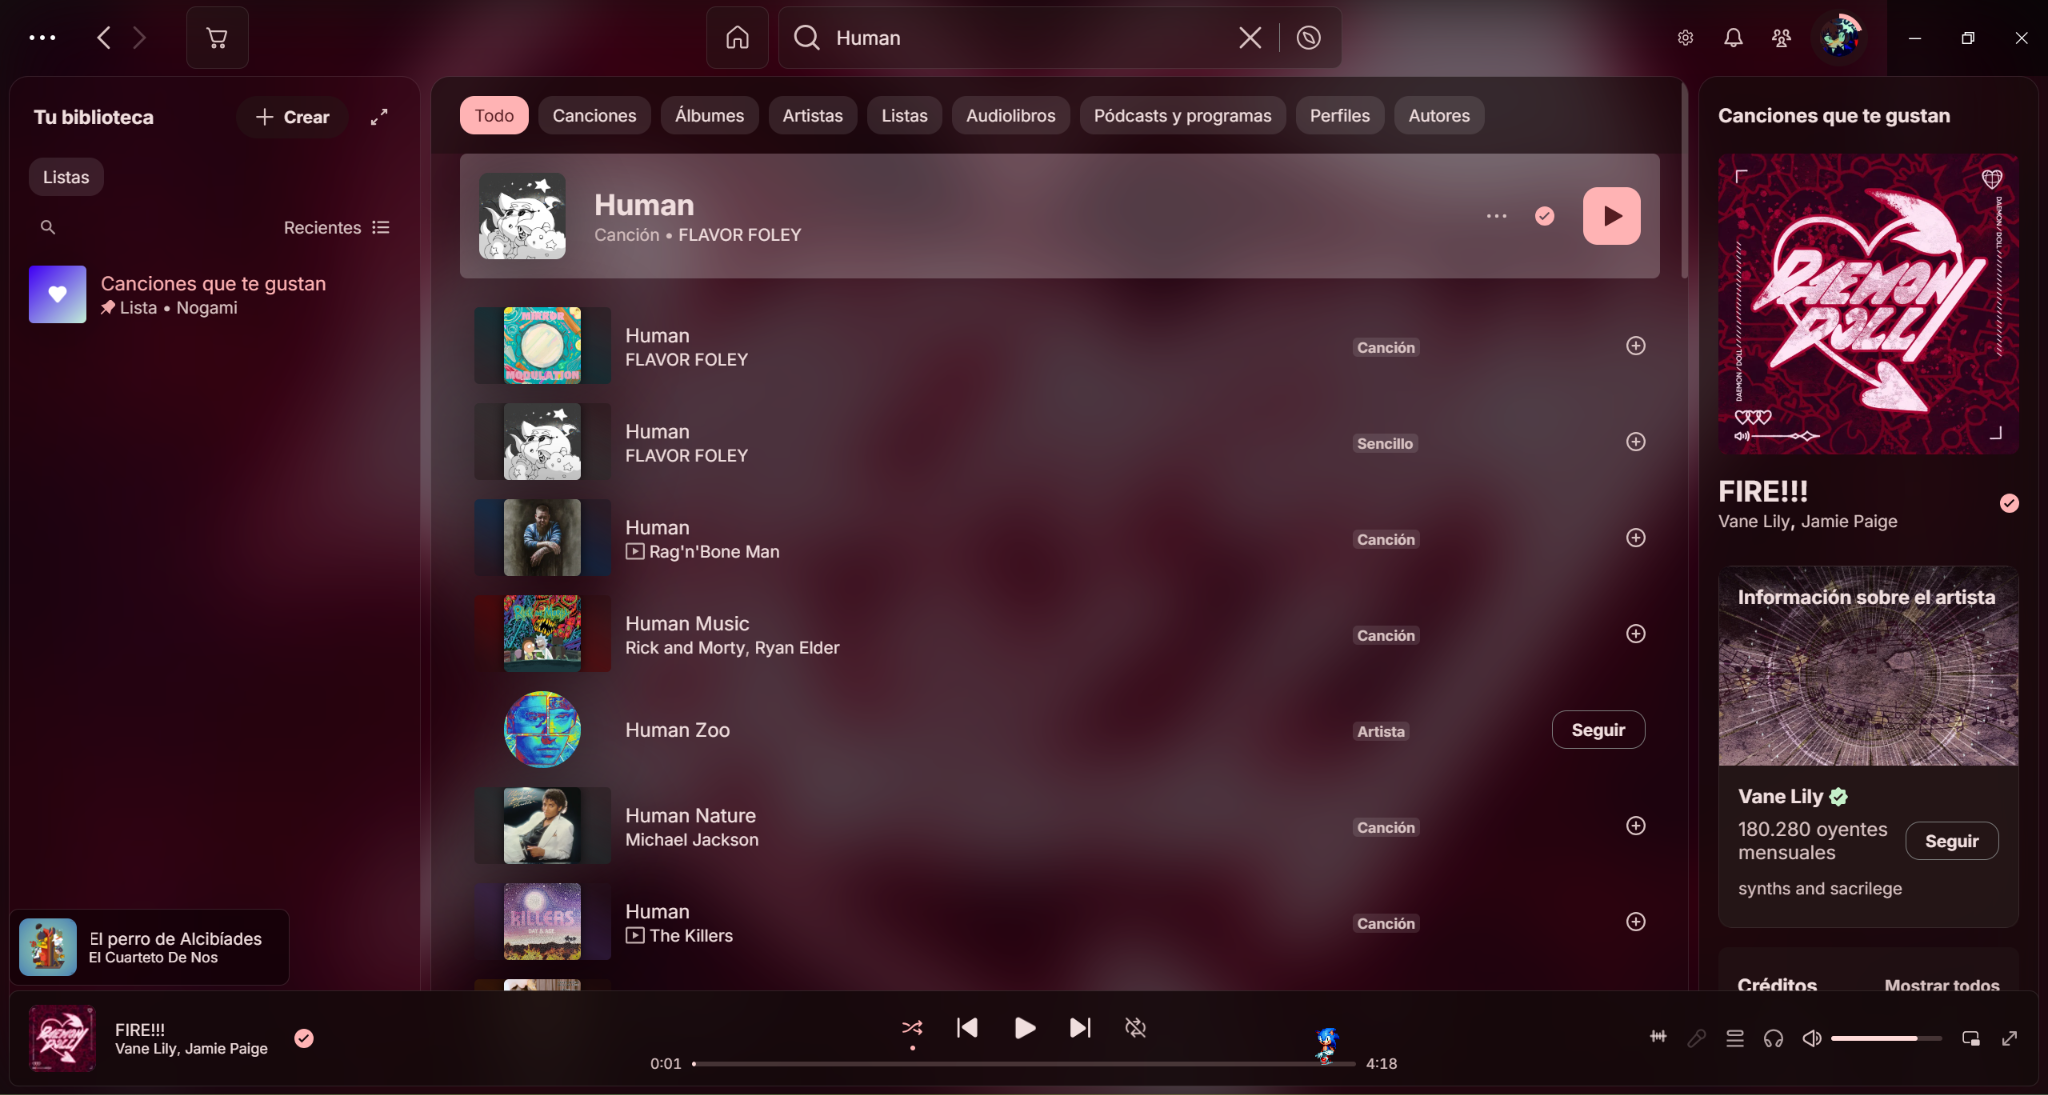
\includegraphics[width=.72\linewidth]{figuras/busqueda_spotify.png}
\captionof{figure}{Búsqueda de «Human» y resultados visibles en Spotify. Fuente: captura del estudiante.}\label{fig:busqueda}
\end{center}
\begin{center}
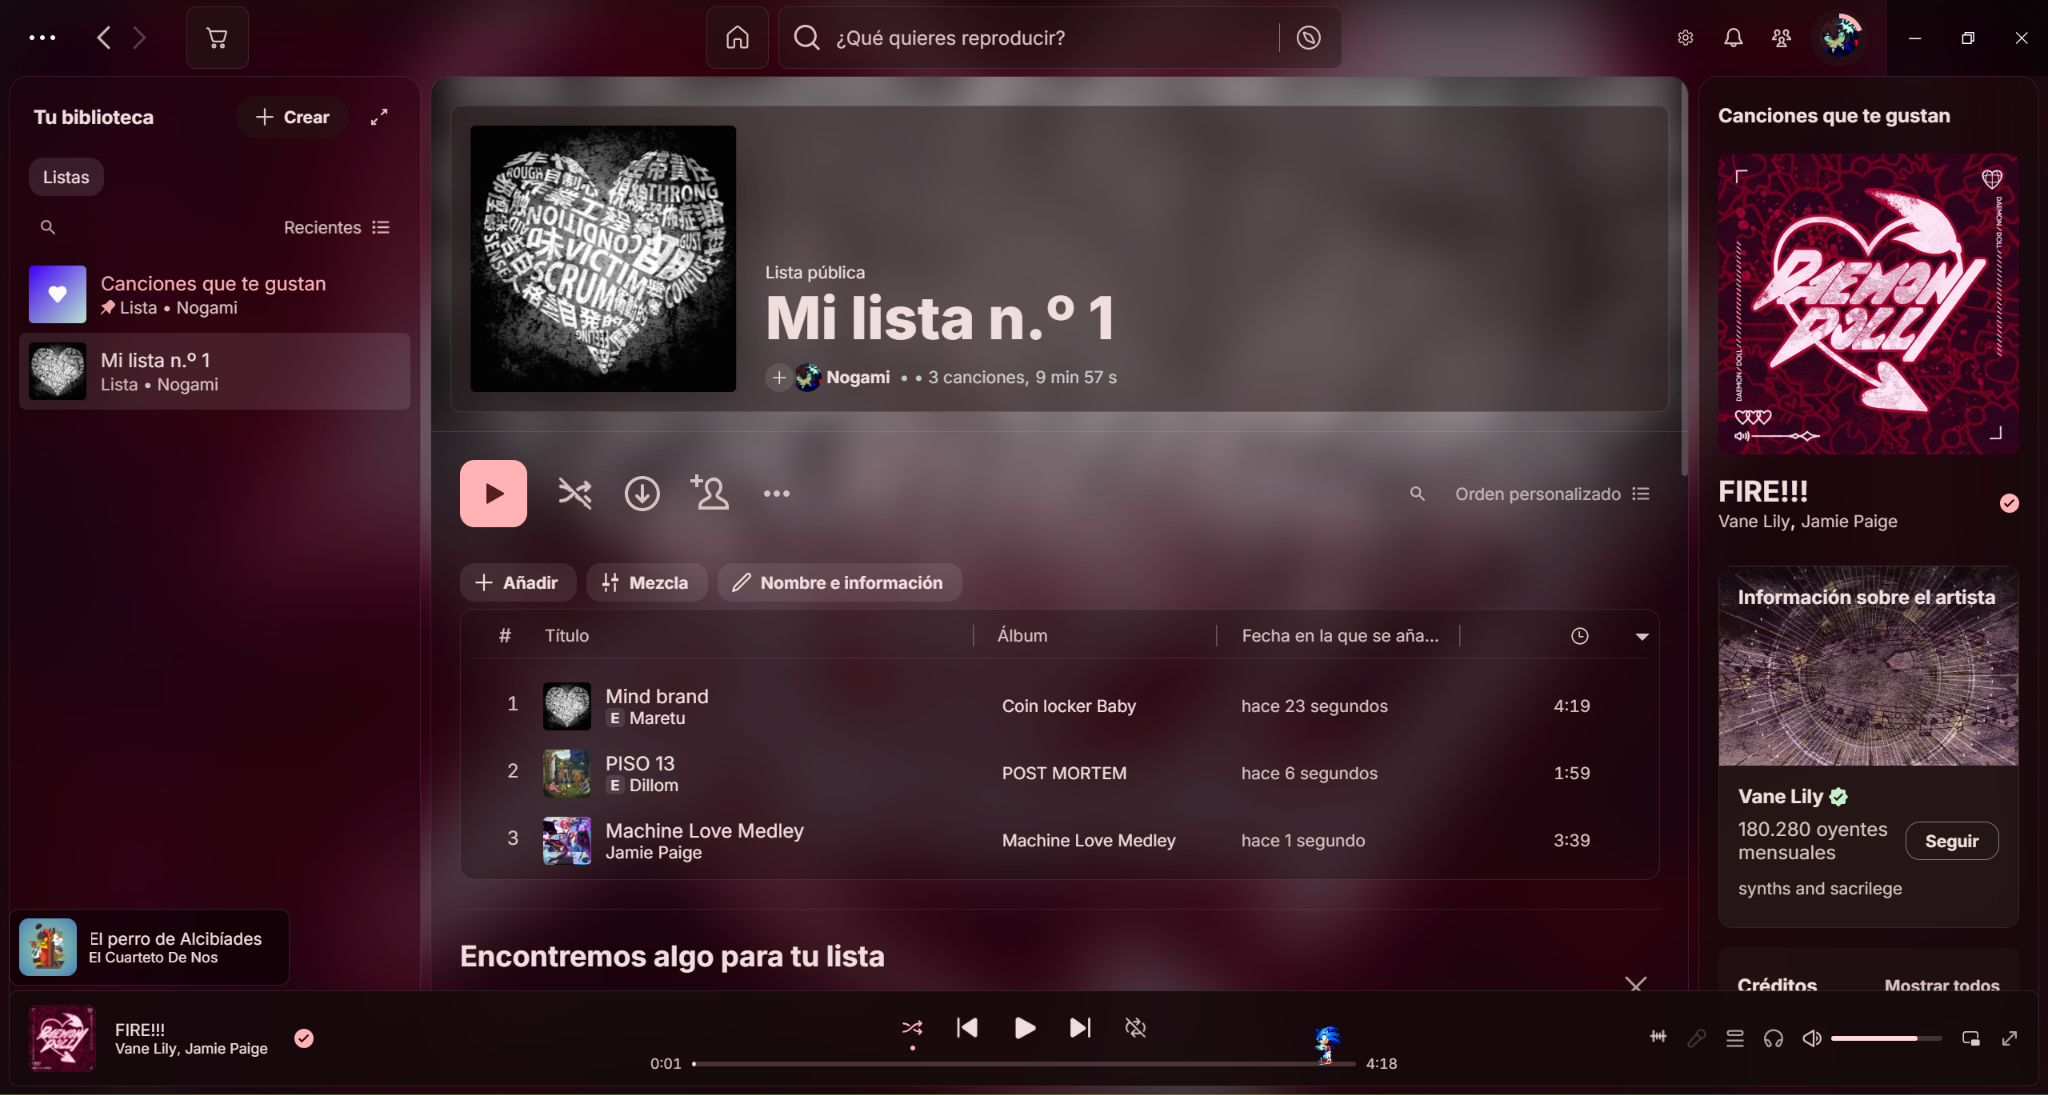
\includegraphics[width=.72\linewidth]{figuras/playlist_spotify.png}
\captionof{figure}{Lista propia con tres canciones. Fuente: captura del estudiante.}\label{fig:playlist}
\end{center}
\begin{center}
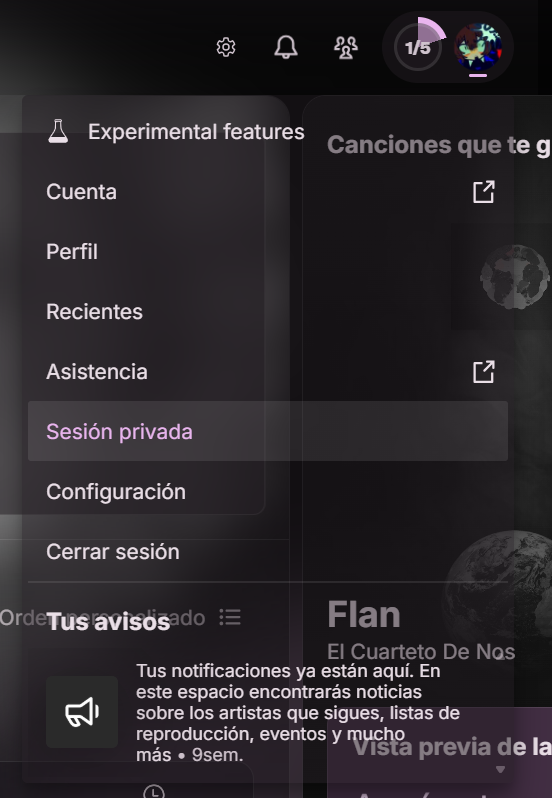
\includegraphics[height=51mm,keepaspectratio]{figuras/sesion_privada_spotify.png}
\captionof{figure}{Opción «Sesión privada» visible en el menú del perfil. Fuente: captura del estudiante.}\label{fig:privada}
\end{center}
\noindent\textbf{Alcance de la evidencia:} Figura~\ref{fig:busqueda} respalda visualmente R-04; Figura~\ref{fig:playlist} respalda la existencia del estado final de R-01 y R-02; Figura~\ref{fig:privada} respalda la disponibilidad del control relacionado con R-14, no su eficacia. Los cinco umbrales cuantitativos (R-11 a R-15) son \textbf{criterios de aceptación propuestos y pendientes de ensayo}, no resultados experimentales.


\section{Reflexión crítica}
La formulación de los requisitos de calidad plantea una dificultad mayor que la descripción de las funciones de búsqueda y gestión de listas: exige transformar expresiones generales en obligaciones medibles. Un ejemplo es pasar de «la búsqueda será muy rápida» a una condición con número de consultas, límite de tiempo y entorno de medición (R-11). Aunque la segunda versión es más verificable, el umbral de tres segundos todavía debe justificarse mediante necesidades de usuarios o criterios del proyecto. Lo mismo ocurre con la privacidad: la presencia de «Sesión privada» en el menú permite identificar la función, pero no comprobar que la actividad quede oculta (Figura~\ref{fig:privada}). Para demostrarlo haría falta un protocolo con cuentas autorizadas y registros de resultados.

El ejercicio diferencia tres niveles de evidencia que no conviene confundir: una captura muestra un estado de la interfaz, una prueba funcional comprueba una operación y una prueba de calidad mide una propiedad bajo condiciones definidas. Además, los requisitos se deben revisar como conjunto para evitar conflictos, por ejemplo entre permisos de las cuentas Free y Premium. El principal aprendizaje técnico consiste en no confundir un requisito redactado con precisión con uno ya validado o cumplido. Esta reflexión describe hallazgos del análisis documental; el estudiante debe revisarla y agregar sus propias dificultades antes de atribuírsela como experiencia personal.


\section{Uso de herramientas de inteligencia artificial}
Se utilizó \textbf{ChatGPT (OpenAI, GPT-6)} para producir y revisar un borrador de texto, ejemplos de requisitos, tablas y código LaTeX; se contrastaron apartados de ISO/IEC/IEEE 29148:2018, ISO/IEC 25010:2023 y las páginas de ayuda de Spotify con fuentes publicadas. Las tres capturas proceden del estudiante. Se comprobó que los archivos LaTeX compilan, pero no se realizaron pruebas cronometradas, entrevistas ni validaciones con usuarios. \textbf{El estudiante debe revisar y editar personalmente el contenido, explicar las decisiones, adaptar la reflexión y verificar todas las referencias antes de presentarlo.}


\begingroup\footnotesize\sloppy\printbibliography[title={Referencias (estilo IEEE)}]\endgroup
\end{document}
